\documentclass[a4paper, 10pt]{article}

% ------------------------------------------------------------------
% Imports
% ------------------------------------------------------------------

% Formatting
\usepackage[landscape, left=0.75cm, top=1.0cm, right=0.75cm, bottom=1.5cm, footskip=15pt]{geometry}
\setlength{\columnsep}{0.5cm}
\usepackage{flowfram}
\ffvadjustfalse
\Ncolumn[<9]{3}
\twocolumn[9]
\usepackage[compact]{titlesec}
\usepackage{parskip}
\setlength{\parskip}{3pt}

% Language stuff
\usepackage[english]{babel}
\usepackage[utf8]{inputenc}

% Math imports
\usepackage{amsthm}
\usepackage{amssymb}
\usepackage{amsmath}
\usepackage{bm}
\usepackage{centernot}
\usepackage{esint}
\usepackage{mathtools}

% Colored boxes
\usepackage{xcolor}
\usepackage{mdframed}
\usepackage{framed}

% Fix for MDFramed
\makeatletter
\DeclareDocumentCommand{\mdtheorem}{ O{} m o m o }%
 {\ifcsdef{#2}%
   {\mdf@PackageWarning{Environment #2 already exits\MessageBreak}}%
   {%
    \IfNoValueTF {#3}%
     {%#3 not given -- number relationship
      \IfNoValueTF {#5}%
        {%#3+#5 not given
        \@definecounter{#2}%
        \expandafter\xdef\csname the#2\endcsname{\@thmcounter{#2}}%
        \newenvironment{#2}[1][]{%
          \refstepcounter{#2}%
          \ifstrempty{##1}%
            {\let\@temptitle\relax}%
            {%
             \def\@temptitle{\mdf@theoremseparator%
                             \mdf@theoremspace%
                             \mdf@theoremtitlefont%
                             ##1}%
             \mdf@thm@caption{#2}{{#4}{\csname the#2\endcsname}{##1}}%
             }%
          \begin{mdframed}[#1,frametitle={\strut#4\ \csname the#2\endcsname%
                                          \@temptitle}]}%
          {\end{mdframed}}%
        \newenvironment{#2*}[1][]{%
          \ifstrempty{##1}{\let\@temptitle\relax}{\def\@temptitle{\mdf@theoremseparator \mdf@theoremspace ##1}}% <- the problem was here
          \begin{mdframed}[#1,frametitle={\strut#4\@temptitle}]}%
          {\end{mdframed}}%
        }%
        {%#5 given -- reset counter
        \@definecounter{#2}\@newctr{#2}[#5]%
        \expandafter\xdef\csname the#2\endcsname{\@thmcounter{#2}}%
        \expandafter\xdef\csname the#2\endcsname{%
               \expandafter\noexpand\csname the#5\endcsname \@thmcountersep%
                  \@thmcounter{#2}}%
        \newenvironment{#2}[1][]{%
          \refstepcounter{#2}%
          \ifstrempty{##1}%
            {\let\@temptitle\relax}%
            {%
             \def\@temptitle{\mdf@theoremseparator%
                             \mdf@theoremspace%
                             \mdf@theoremtitlefont%
                             ##1}%
             \mdf@thm@caption{#2}{{#4}{\csname the#2\endcsname}{##1}}%
             }
          \begin{mdframed}[#1,frametitle={\strut#4\ \csname the#2\endcsname%
                                          \@temptitle}]}%
          {\end{mdframed}}%
        \newenvironment{#2*}[1][]{%
          \ifstrempty{##1}%
            {\let\@temptitle\relax}%
            {%
             \def\@temptitle{\mdf@theoremseparator%
                             \mdf@theoremspace%
                             \mdf@theoremtitlefont%
                             ##1}%
             \mdf@thm@caption{#2}{{#4}{\csname the#2\endcsname}{##1}}%
             }%
          \begin{mdframed}[#1,frametitle={\strut#4\@temptitle}]}%
          {\end{mdframed}}%
        }%
     }%
     {%#3 given -- number relationship
        \global\@namedef{the#2}{\@nameuse{the#3}}%
        \newenvironment{#2}[1][]{%
          \refstepcounter{#3}%
          \ifstrempty{##1}%
            {\let\@temptitle\relax}%
            {%
             \def\@temptitle{\mdf@theoremseparator%
                             \mdf@theoremspace%
                             \mdf@theoremtitlefont%
                             ##1}%
             \mdf@thm@caption{#2}{{#4}{\csname the#2\endcsname}{##1}}%
             }
          \begin{mdframed}[#1,frametitle={\strut#4\ \csname the#2\endcsname%
                                          \@temptitle}]}%
          {\end{mdframed}}%
        \newenvironment{#2*}[1][]{%
          \ifstrempty{##1}{\let\@temptitle\relax}{\def\@temptitle{:\ ##1}}%
          \begin{mdframed}[#1,frametitle={\strut#4\@temptitle}]}%
          {\end{mdframed}}%
     }%
   }%
 }
\makeatother

% Tables
\usepackage{tabularx} % tabularx since the width should be handled automatically
\usepackage{booktabs}
\usepackage{makecell}

% Graphics
\usepackage{pgfplots}
\usepackage{physics}
\usepackage{tikz}
\usepackage{tikz-3dplot}
\usepackage{graphics}
\usetikzlibrary{arrows, matrix, angles, quotes, intersections}

% Miscellaneous
\usepackage{hyperref}
\usepackage{enumerate}
\usepackage{enumitem}
\usepackage{multicol}

% ------------------------------------------------------------------
% Formatting
% ------------------------------------------------------------------
\mdfsetup{skipabove=5pt,skipbelow=5pt}
\hypersetup{colorlinks=true, urlcolor=blue, linkcolor=blue, citecolor=blue}
\setlist{itemsep=0.5pt, topsep=0.5pt, leftmargin=6mm}
\renewcommand{\labelenumii}{\arabic{enumi}.\arabic{enumii}}

% Change the top/bottom margin of math environment
\makeatletter
\g@addto@macro\normalsize{%
  \setlength\abovedisplayskip{4pt}
  \setlength\belowdisplayskip{4pt}
  \setlength\abovedisplayshortskip{4pt}
  \setlength\belowdisplayshortskip{4pt}
}
\makeatother

% Theorems and Styles
% ------------------------------------------------------------------
% Colors
% ------------------------------------------------------------------
\definecolor{general}{HTML}{333333}
\definecolor{discrete_highlight}{HTML}{8B6CEF}
\definecolor{cont_highlight}{HTML}{2ECC71}
\definecolor{cont_bg}{HTML}{2f2f2f}

% ------------------------------------------------------------------
% Color Boxes Formatting
% ------------------------------------------------------------------
\mdfsetup{
  linecolor=general,
  linewidth=3pt,
  topline=false,
  bottomline=false,
  rightline=false,
  innertopmargin=5pt,
  innerbottommargin=5pt,
  innerrightmargin=5pt,
  innerleftmargin=5pt,
  leftmargin=0pt,
  rightmargin=0pt,
  frametitleaboveskip=2pt,
  frametitlebelowskip=2pt,
  theoremseparator={},
  theoremspace={},
}

\mdfdefinestyle{discrete_definition}{
  linecolor=discrete_highlight,
  backgroundcolor=gray!20,
  frametitlebackgroundcolor=gray!30,
}

\mdfdefinestyle{discrete_theorem}{
  linecolor=discrete_highlight,
  innertopmargin=0pt,
}

\mdfdefinestyle{cont_definition}{
  linecolor=cont_highlight,
  backgroundcolor=gray!20,
  frametitlebackgroundcolor=gray!30,
}

\mdfdefinestyle{cont_theorem}{
  linecolor=cont_highlight,
  innertopmargin=0pt,
}

\mdfdefinestyle{definition}{
  backgroundcolor=gray!20,
  frametitlebackgroundcolor=gray!30,
}

\mdfdefinestyle{theorem}{
  innertopmargin=0pt,
}

\mdfdefinestyle{note}{
  leftline=false,
  backgroundcolor=gray!20,
  frametitlebackgroundcolor=gray!30,
}

% ------------------------------------------------------------------
% Custom Commands
% ------------------------------------------------------------------

% Normal theorem environments
\newtheorem*{corollary}{Cor}
\newtheorem*{lemma}{Lemma}
\newtheorem*{proposition}{Proposition}

% Colored theorem environments
\mdtheorem[style=discrete_theorem]{dtheorem}{}
\mdtheorem[style=discrete_definition]{ddefinition}{}
\mdtheorem[style=cont_theorem]{ctheorem}{}
\mdtheorem[style=cont_definition]{cdefinition}{}
\mdtheorem[style=theorem]{theorem}{}
\mdtheorem[style=definition]{definition}{}
\mdtheorem[style=note]{note}{}

% ------------------------------------------------------------------
% Custom Commands
% ------------------------------------------------------------------

% Math general
\newcommand{\R}{\mathbb{R}}
\newcommand{\Q}{\mathbb{Q}}
\newcommand{\N}{\mathbb{N}}
\newcommand{\Z}{\mathbb{Z}}
\newcommand{\C}{\mathbb{C}}
\newcommand{\Pow}{\mathcal{P}}

% Probability Stuff
\renewcommand{\O}{\Omega}
\renewcommand{\P}{\mathbb{P}}
\newcommand{\E}{\mathbb{E}}
\newcommand{\F}{\mathcal{F}}
\newcommand{\B}{\mathcal{B}}
\newcommand{\I}{1}
\renewcommand{\L}{\mathcal{L}}
\DeclareMathOperator{\Var}{Var}
\DeclareMathOperator{\Cov}{Cov}
\DeclareMathOperator{\Ber}{Ber}
\DeclareMathOperator{\Bin}{Bin}
\DeclareMathOperator{\NB}{NB}
\DeclareMathOperator{\Geom}{Geom}
\DeclareMathOperator{\Cat}{Cat}
\DeclareMathOperator{\Poisson}{Poisson}
\DeclareMathOperator{\Unif}{\mathcal{U}}
\DeclareMathOperator{\Exp}{Exp}
\DeclareMathOperator{\Normal}{\mathcal{N}}
\DeclareMathOperator{\Ga}{Ga}
\DeclareMathOperator{\Atom}{Atom}
\DeclareMathOperator{\DX}{\mathcal{X}}

% Statistical stuff
\DeclareMathOperator{\MSE}{MSE}
\DeclareMathOperator{\MLE}{MLE}
\DeclareMathOperator{\ML}{ML}

% Misc
\newcommand{\sdots}{\ifmmode\mathinner{\ldotp\kern-0.2em\ldotp\kern-0.2em\ldotp}\else.\kern-0.13em.\kern-0.13em.\fi}

% ------------------------------------------------------------------
% Meta Data
% ------------------------------------------------------------------
\title{\vspace{-3ex}Probability and Statistics}
\author{Nicola Studer \\ \href{mailto:nicstuder@student.ethz.ch}{nicstuder@student.ethz.ch}}
\date{\vspace{-5ex}}


% ------------------------
% Document
% ------------------------

\begin{document}

% Title
\maketitle
\begin{align*}
  \color{general} \blacksquare \ & \text{General} & \color{discrete_highlight} \blacksquare \ & \text{Discrete} & \color{cont_highlight} \blacksquare \ & \text{Continuous}
\end{align*}

% Sections
\section{Mathematical framework}

\begin{definition*}[Probability Space \((\O, \F, \P)\)]
  \begin{itemize}
    \item \(\bm{\O} \neq \emptyset\): \textbf{Sample space} with \(\omega \in \O\) as outcome.
    \item \(\bm{\F}\subseteq \Pow(\O)\): \textbf{\(\bm{\sigma}\)-algebra}
    \begin{enumerate}
      \item \(\Omega \in \F\)
      \item \(A \in \F \implies A^\complement \in \F\) where \(A\) is an event.
      \item \(A_1, A_2, \ldots \in \F \implies \bigcup_{i=1}^\infty \in \F\)
    \end{enumerate}
    \item \(\pmb{\P}\): \textbf{Probability measure} on \((\O, \F)\)
    \begin{enumerate}
      \item[\(\P:\)] \(\F \to [0, 1], A \mapsto \P(A)\)
      \item \(\P(\O) = \sum_{\omega \in \O} p(\omega) = 1\) if \(p(\omega) := \P(\{\omega\})\).
      \item \(P(A) = \sum_{i=1}^\infty P(A_i)\) if \(A = \bigcup_{i=1}^\infty A_i\) disjoint.
    \end{enumerate}
  \end{itemize}
\end{definition*}

We have some further consequences of this definition:
\begin{enumerate}
  \item \(\emptyset \in \F\)
  \item \(A_1, \ldots \in \F \Rightarrow \bigcap_{i=1}^\infty A_i \in \F\)
  \item \(A, B \in \F \implies A \cup B \in \F\)
  \item \(A, B \in \F \implies A \cap B \in \F\)
\end{enumerate}

and

\begin{enumerate}
  \item \(\P(\emptyset) = 0\)
  \item \(\P(A^\complement) = 1 - \P(A)\)
  \item \(\P(A \cup B) = \P(A) + \P(B) - \P(A \cap B)\)
  \item \(A_1, \ldots A_k\) disjoint \(\implies \P(\bigcup_{i=1}^k A_i) = \sum_{i=1}^k \P(A_i)\)
  \item \(\P(\bigcup_{i=1}^k A_i) = \sum_{i=1}^k \sum_{1 \leq j_1 < \ldots < j_i \leq k} \P(A_{j_1} \cap \ldots \cap A_{j_i})\)
  \item (Union Bound) \(\P(\bigcup_{i=1}^\infty A_i) \leq \sum_{i=1}^\infty \P(A_i)\)
  \item (Monotonicity) \(A \subseteq B \implies \P(A) \leq \P(B)\)
  \item (De Morgan's Law) \((\bigcup_{i=1}^\infty A_i)^\complement = \bigcap_{i=1}^\infty (A_i)^\complement\)
  \item \(A \setminus (A \cap B^\complement) = A \cap B\)
\end{enumerate}

 \pagebreak
\section{Conditional probabilities}

\begin{definition*}[Conditional probability]
  Let \((\O, \F, \P)\) be some probability space and \(A, B \in \F\) with \(\P(B) > 0\). Then the \textbf{conditional probability of \(A\) given \(B\)} is defined by:
  \[\P(A \mid B) = \frac{\P(A \cap B)}{\P(B)}\]
\end{definition*}

\begin{proposition}
  Let \((\O, \F, \P)\) be some probability space and \(B \in \F\). then \(\P(\cdot \mid B)\) is a probability measure on \((\O, \F)\).
\end{proposition}

\begin{theorem*}[Law of total probability]
  Let \(\B = (B_i)_{i \in I}\) be a countable partition of \(\O\). Then
  \[\forall A \in \F \quad \P(A) = \sum_{i \in I: \P(B_i) > 0} \P(A \mid B_i) \cdot \P(B_i)\]
\end{theorem*}

\begin{theorem*}[Chain Rule of Probability]
  If \(\P(\bigcap_{i=1}^n A_i) > 0\), then we can write it as:
 \[ \P(\cap_{i=1}^n A_i) = \P(A_1) \P(A_2 \mid A_1) \cdots \P(A_n \mid A_1 \cap \ldots \cap A_{n-1})\]
\end{theorem*}

\begin{theorem*}[Bayes' theorem]
  Let \(\B = (B_i)_{i \in I}\) be a countable partition of \(\O\) where \(\P(B_i) > 0\) for all \(i\). Then for all \(A \in \F\) with \(\P(A) > 0\):
  \[\P(B_i \mid A) = \frac{\P(A \mid B_i) \cdot \P(B_i)}{\sum_{j \in I} \P(A \mid B_j) \cdot \P(B_j)}\]
\end{theorem*}


\section{Independence}
\begin{ddefinition*}[Independence of two events]
  Let \((\O, \F, \P)\) be a probability space. A collection of events \(A_1, \ldots, A_n\) is called independent, if
  \[\forall I \subseteq \{1, \ldots, n\} \quad \P\left(\bigcap_{i \in I} A_i\right) = \prod_{i \in I} \P(A_i)\]
\end{ddefinition*}
\[A, B \ \text{ind.} \iff \P(A \mid B) = \P(A) \iff \P(B \mid A) = \P(B)\]

\begin{itemize}
  \item If \(A, B\) are independent, then likewise \(A, B^\complement\).
  \item \(\P(A) \in \{0, 1\} \implies A\) is independent for all events.
  \item If \(A\) is independent of itself, then \(\P(A) \in \{0, 1\}\)
\end{itemize}


\section{Random variables}

Let \((\O, \F, \P)\) be a probability space. A random variable is \textbf{measurable} map \(X: \Omega \to \R\)  such that for all \(a \in \R\):
\[\{\omega \in \O \mid X(\omega) \leq a\} \in \F\]

Furthermore we can define \textbf{events} in terms of a \textbf{random variable} where we use an abuse of notation:
\[\{X \leq a\} = \{\omega \in \O \mid X(\omega) \leq a\}\]
Which has a probability of \(\P(X \leq a) = \P(\{X \leq a\})\).

\begin{definition*}[Preimage of a random variable \(X\)] \vspace{-5pt}
  \[X^{-1}(A) = \{\omega \in \O \mid X(\omega) \in A\} = \bm{"X \in A"} \quad A \subset \R\]
  \(X\) is \textbf{\(\bm{\F}\)-measurable} if \(\forall B \subsetneq \R\), \(B\) closed: \(X^{-1}(B) \in \F\).
\end{definition*}

\begin{definition*}[Distribution of a Random Variable]
  For \(A \in \B(\R)\), we define the distribution (\textbf{law}) of \(X\) as
  \[\mu(A) = \P_X(A) := \P(X^{-1}(A)) = \P(\{\omega \in \O \mid X(\omega) \in A\})\]
\end{definition*}

\begin{definition*}[Cumulative Distribution Function (CDF)]
  Let \(X\) be a random variable on the probability space \((\O, \F, \P)\), the CDF \(F_X: \R \to [0, 1]\) is defined by
  \[\forall x \in \R \quad F_X(x) = \P(X^{-1}((-\infty, x))) =:\P(X \leq x) \]
\end{definition*}
Properties of the CDF (characterized by RCLL, Càdlàg):
\begin{itemize}
  \item \(a < b \implies \P(a < X \leq b) = F_X(b) - F_x(a)\)
  \item \(F_X\) is monotonically increasing
  \item \(F_X\) is right-continuous, i.e. \(\lim_{y \to x^+} F_X(y) = F_X(x)\)
  \item \(\lim_{x \to -\infty} F_X (x) = 0\) and \(\lim_{x \to \infty} F_X(x) = 1\)
\end{itemize}

\begin{definition*}[Independence of random variables]
  The RVs \(X_1, \ldots, X_n\) are called independent, if
  \begin{align*}
    \forall x_1, \ldots, x_n \in \R: \quad & \P(X_1 \leq x_1, \ldots, X_n \leq x_n) = \\
    & \P(X_1 \leq x_1) \cdot \ldots \cdot \P(X_n \leq x_n)
  \end{align*}
\end{definition*}

\pagebreak
\subsection{Discrete random variables}
A random variable \(X\) is called \textbf{discrete} if the set of values it can output \(\DX\), is a discrete (a finite or countable set).

\begin{ddefinition*}[Probability Mass Function (PMF)]
  Let \(X\) be a discrete random variable and \(\DX\) be the set of all its values. The probability mass function \(p_x(x)\) for each \(x \in \DX\) is defined by:
  \[p_X(x) = \P(X = x) = \P_X(\{x\}) = \P(X^{-1}(\{x\}))\]
\end{ddefinition*}

\begin{ddefinition*}[CDF of a discrete random variable] \vspace{-5pt}
  \[F_X(x) = \P(X \leq x) = \sum_{x' \in \DX \leq x} p_X(x')\]
\end{ddefinition*}

\subsection{Continuous Random Variable}
A random variable \(X\) is called \textbf{continuous} if the set of values it can produce is uncountably infinite and the probability of attaining a single value is zero.

\begin{cdefinition*}[Probability Density Function (PDF)]
  Let \(X\) be a continuous random variable. If there exists a (measureable) function \(f_x: \R \to [0, \infty)\), such that
  \[\P_X(I) = \P(X \in I) = \int_I f_x(x) \,dx\]
  for all intervals \(I\) in \(\R\), we call it the \textbf{PDF}.
\end{cdefinition*}

Notice that \(\int_\R f_x(x) \, dx = 1\) since \(\P_X(\R) = 1\).

\begin{cdefinition*}[CDF of a continuous random variable] \vspace{-5pt}
  \[F_x(x) = \P(X \leq x) = \int_{-\infty}^x f_x(t) \,dt = \P_X((-\infty, x])\]
\end{cdefinition*}
The definition leads to the following consequences:
\begin{itemize}
  \item \(\P(a \leq x \leq b) = \P(a < x < b)\)
  \item \(\P(X = x) = 0\)
  \item \(\P(X \in [a, b]) = \P(X \in (a, b))\)
  \item \(F_x\) differentiable \(\implies \frac{dF_x}{dx}(x_0) = f_x(x_0)\)
\end{itemize}

\section{Expectation}

For any random variable \(X: \Omega \to \R_+\) with non-negative values, the expected value is defined with the CDF as:
\[\E(X) = \int_\R x \,dF_X(x) \color{gray!70} = \int_\R x \frac{F_X(x)}{dx} \, dx\]

\begin{ddefinition*}[Expected Value, Discrete]
  Let \(X\) be a discrete random variable with value in \(\DX\). The expected value is defined as (if the sum is well defined):
  \[\E(X) := \sum_{x \in \DX}x \cdot p_X(x) = \sum_{\omega \in \O} X(\omega) \cdot p(\omega)\]
\end{ddefinition*}

\begin{proposition}
  {\small \(\E(\I_A) = \P(A)\)}.
\end{proposition}

\begin{proposition}
  If \(\DX \subseteq \N_0\), then \(\E(X) = \sum_{j=0}^\infty \P(X > j)\).
\end{proposition}

\begin{dtheorem*}[Law of the unconscious statistician (LOTUS)] \vspace{-5pt}
  \[\E(\phi(X)) = \sum_{x \in \DX}\phi(x) \cdot p_X(x)\]
\end{dtheorem*}

\begin{cdefinition*}[Expected Value, Continuous]
  Let \(X\) be a continuous random variable with density \(f_x\). The expected value is defined as:
  \[\E(X) := \int_{\R} x \cdot f_X(x) \,dx\]
\end{cdefinition*}

\begin{ctheorem*}[LOTUS] \vspace{-5pt}
  \[\E(\phi(X)) = \int_\R \phi(x) \cdot f_X(x) \, dx\]
\end{ctheorem*}

\begin{theorem*}[Linearity of expected value] \vspace{-5pt}
  \[\E(\alpha X + \beta Y) = \alpha \E(X) + \beta \E(Y) \quad (a, b \in \R)\]
\end{theorem*}

\begin{theorem*}[Expected value of \(XY\), independence] \vspace{-5pt}
  \[X, Y \ \text{ind.} \Leftrightarrow \E(\phi(X) \psi(Y)) = \E(\phi(X)) \E(\psi(Y))\]
\end{theorem*}
This theorem also holds for \(X_1, \ldots X_n\) and \(\phi_1, \ldots, \phi_n\).

\pagebreak
\subsection{Variance and Covariance}
\begin{definition*}[Variance]
  Let \(X\) be a random variable such that \(\E(X^2) < \infty\). The variance of \(X\) is defined as:
  \[\Var(X) = \sigma_X^2 = \E((X - \E(X))^2) = \E(X^2) - \E(X)^2\]
  \(\sigma_X\) is called the \textbf{standard deviation} of \(X\).
\end{definition*}

\begin{itemize}
  \item If \(\E(X^2) < \infty, \lambda, \alpha \in \R\), then \(\Var(\lambda X + \alpha) = \lambda^2 \Var(X)\).
  \item If \(S = X_1 + \ldots + X_n\), with \(X_1, \ldots, X_n\) pairwise independent (or uncorrelated), then \(\sigma_S^2 = \sum_{i = 1}^n \sigma_{X_i}^2\)
\end{itemize}

\begin{definition*}[Covariance]
  Let \(X, Y\) be two random variables with \(\E(X^2) < \infty\) and \(\E(Y^2) < \infty\), then their covariance is defined as
  \[\Cov(X, Y) = \E((X - \E(X))(Y - \E(Y)))\]
  If \(\Cov(X, Y) = 0\), then they are uncorrelated.
\end{definition*}
\begin{itemize}
  \item \(\Cov(X, X) = \sigma_X^2 = \Var(X)\)
  \item \(X, Y\) independent \(\implies \Cov(X, Y) = 0\)
\end{itemize}

\subsection{Inequalities}
\begin{lemma}[Monotonicity]
  \(X \leq Y \implies \E(X) \leq \E(Y)\)
\end{lemma}

\begin{theorem*}[Markov's Inequality]
  Let \(X\) be a R.V, \(g: \DX \to [0, \infty)\) monotonically increasing, then for \(a \in \R\):
  \[\P(X \geq a) \leq \frac{\E(g(X))}{g(a)}\]
\end{theorem*}

\begin{theorem*}[Jensen's Inequality]
  Let \(X\) be a R.V, \(\phi: \R \to \R\) a convex function, then
  \[\phi(\E(X)) \leq \E(\phi(X))\]
\end{theorem*}

\begin{theorem*}[Chebychev's Inequality]
  Let \(X\) be a R.V. s.t. \(\E(X^2) < \infty\), then for \(t > 0\)
  \[\P(|X - \E(X)| \geq t) \leq \frac{\Var(X)}{t^2}\]
\end{theorem*}
 \pagebreak
\section{Joint Distributions}
\begin{definition*}[Joint Distribution]
  Let \(X_1, \ldots, X_n\) be R.V. defined on the same probability space \((\O, \F, \P)\). Consider \(X = (X_1, \ldots, X_n)\). The joint distribution \(\P_X\) on the hyper set \(A \in \B^n\) where \(\B^n = \sigma(\{A_1 \times \cdots \times A_n \mid A_i \in \B\})\) is defined as:
  \[\P_X(A) = \P(X^{-1}(A)) = \P(\{\omega \in \O \mid X(\omega) \in A\})\]
\end{definition*}

\begin{ddefinition*}[Joint PMF]
  Let \(X = X_1, \ldots, X_n\) be discrete R.V., defined on the same probability space.
  \[p_{X}(x_1, \ldots, x_n) = \P(X_1 = x_1, \ldots, X_n = x_n)\]
\end{ddefinition*}

\begin{ddefinition*}[Joint CDF, discrete]
  Let \(X = X_1, \ldots, X_n\) be discrete R.V., defined on the same probability space.
  \[\scriptstyle F_X(x_1, \ldots, x_n) = \P(X_1 \leq x_1, \ldots, X_n \leq x_n) = \smashoperator{\sum_{y_1 \leq x_1, \ldots, y_n \leq x_n}} p(y_1, \ldots, y_n)\]
\end{ddefinition*}

\begin{proposition}
  Let \(X_1, \ldots X_n\) be discrete R.V. with \(X_i \in \DX_i\). Then \(Z = \phi(X_1, \ldots, X_n)\) is a discrete random variable with values in \(\DX = (\DX_1 \times \ldots \times \DX_n)\) and with distribution given by \(\forall z \in \DX\):
  \[\P(Z = z) = \sum_{\substack{x_1 \in \DX_1, \ldots, x_n \in \DX_n \\ \phi(x_1, \ldots, x_n) = z}} \P(X_1 = x_1, \ldots, X_n = x_n)\]
\end{proposition}

\begin{dtheorem*}[Marginal distribution, discrete]
  Let \(X_1, \ldots, X_n\) be discrete R.V. with joint PMF. For every \(i\) we have \(\forall z \in \DX_i\):
  \[\P(X_i = z) = \smashoperator[r]{\sum_{x_1, \ldots x_{i-1}, x_{i+1}, \ldots, x_n}} p(x_1, \ldots, x_{i-1}, z, x_{x+1}, \ldots, x_n)\]
\end{dtheorem*}

\begin{proposition}
  The expected values of joint discrete R.V. can be written as:
  \[\E(\phi(X_1, \ldots, X_n)) = \smashoperator[r]{\sum_{x_1 \in \DX_1, \ldots, x_n \in \DX_n}} \phi(x_1, \ldots, x_n) \cdot p(x_1, \ldots, x_n)\]
\end{proposition}

\pagebreak
\begin{cdefinition*}[Joint PDF]
  Let the R.V. \(X = X_1, \ldots, X_n\) be defined on the same probability space. We say these R.V. have a joint PDF \(f_{X_1, \ldots, X_n} = f_X\) if for all subsets \(A \in \B^n\) it holds
  \begin{align*}
    \P_X(A) = \P((X_1, \ldots, X_n) \in A) \\
    = \int_A f_X(x_1, \ldots, x_n) \, dx_1 \ldots \,dx_n
  \end{align*}
\end{cdefinition*}

\begin{cdefinition*}[Joint CDF, continuous]
  Let \(X = X_1, \ldots, X_n\) be continuous R.V., defined on the same probability space.
  \begin{align*}
    F_{X}(x_1, \ldots, x_n) = \P(X_1 \leq x_1, \ldots, X_n \leq x_n) \\
    = \int_{-\infty}^{x_1} \ldots \int_{-\infty}^{x_n} f_{X}(x_1, \ldots, x_n) \,dx_n \ldots \, dx_1
  \end{align*}
\end{cdefinition*}

\begin{proposition}
  Let \(X_1, \ldots, X_n\) be continuous R.V. with joint PDF and \(\phi: \R^n \to \R\). The expected value is defined as
  \begin{multline*}
    \E(\phi(X_1, \ldots, X_n)) = \\ \int_\R \ldots \int_\R \phi(x_1, \ldots, x_n) \cdot f(x_1, \ldots, x_n) \, dx_n \ldots \, dx_1
  \end{multline*}
\end{proposition}

\begin{ctheorem*}[Marginal density, continuous]
  Let \(X_1, \ldots, X_n\) be continuous R.V. with a joint PDF. For every \(i\) we have \(\forall z \in \DX_i\):
  \[f_{X_i}(z) = \smashoperator{\int_{x_1, \ldots, x_{i-1}, x_{x+1}, \ldots, x_n}} f(x_1, \ldots, x_{i-1}, z, x_{i+1}, \ldots, x_n) \, dx_n \ldots \, dx_1\]
\end{ctheorem*}

\begin{theorem*}[Independence of joint Random Variables]
  Let \(X_1, \ldots, X_n\) be R.V. with \(p_{X_1}, \ldots, p_{X_n}\).
  \begin{itemize}
    \item[] \(X_1, \ldots X_n\) are independent
    \item[\(\Leftrightarrow\)] \(p(x_1, \ldots, x_n) = p_{X_1}(x_1) \cdot \ldots \cdot p_{X_n}(x_n)\)
    \item[\(\Leftrightarrow\)] \(\E(\phi_1(X_1) \cdot \ldots \cdot \phi_n(X_n)) = \E(\phi_1(X_1)) \cdot \ldots \cdot \E(\phi_n(X_n))\)
  \end{itemize}
\end{theorem*}

\subsection{Useful lemmas and theorems}

\begin{definition*}[Distribution of transformed Random Variables]
  Let \(X = (X_1, \ldots, X_n)\) and \(Y(\omega) = g(X(\omega))\) be two random variable with \(g: \R^n \to \R^m\). Then for any \(A \in \B(\R)\)
  \[\mu_Y(A) = \mu_X(g^{-1}(A)).\]
\end{definition*}

\begin{theorem*}[Transformation Theorem]
  Let \(g(x) = m + Bx\) with \(\det(B) \neq 0\). If \(\mu_X\) is abs. continuous, then \(\mu_Y\) is abs. continuous and furthermore
  \[f_Y(x) = \frac{1}{|\det(B)|} f_X(B^{-1}(x - m)).\]
\end{theorem*}

\begin{example}
  \(X_1, X_2 \sim U(0, 1)\), CDF of \(Y = X_1 + X_2, Z = X_1 - X_2\)? \\
  Then \(g(x_1, x_2) = (x_1 + x_2, x_1 - x_2)\) and \(B = \begin{pmatrix}
    1 & 1 \\
    1 & -1
  \end{pmatrix}\) with \(\det (B) = 2\), \(g(x) = Bx\). Thus \((Y, Z) = g(X_1, X_2)\) and with the transformation theorem we get
  \[f_{Y, Z}(y, z) = f_{X_1, X_2}(g^{-1}(y, z)) = \frac{1}{2}f_{X_1, X_2}\left(\frac{y+z}{2}, \frac{y-z}{2}\right)\]
\end{example}

\begin{proposition}
  If the R.V. \((X, Y)\) has a density function \(f\), then \(Z = X + Y\) has a density 
  \(f_Z(z) = \int_\R f(x, z - x) \, dx\).
\end{proposition}

\begin{definition*}[Convolution]
  If \(X, Y\) indep., then \(Z = X + Y\) has a density function:
  \[(f_X * f_Y) := f_Z(z) = \int_\R f_X(x)f_Y(z - x) \, dx\]
  \[\forall k \in \N_0 : \P[X + Y = k] = \sum_{j=0}^k \P[X = j] \P[Y = k - j]\]
\end{definition*}

\begin{proposition}
  Suppose \(X_1, \ldots, X_n\) are i.i.d with CDF \(F\). Then \(V = \max\{X_1, \ldots, X_n\}\) has CDF \(F_V(x) = F^n(x) \) as \(\P(\max\{X_1, \ldots, X_n\} < x) = \P(X_1 < x, \ldots, X_n < x)\) and
  \(U = \min \{X_1, \ldots, X_n\}\) has CDF \(F_U(x) = 1 - (1 - F(x))^n\).
\end{proposition}

\begin{ctheorem*}[Transformation of Bivariate Random Variables]
  Let \((X, Y)\) be two R.V. with \(f_{X, Y}\). If we have a bijective transformation \(U = g_1(X, Y), V = g_2(X, Y)\) with inverses \(X = h_1(U, V)\) and \(Y = h_2(U, V)\), then:
  \[f_{U, V}(u, v) = f_{X, Y}(h_1(u, v), h_2(u, v))|J| \quad J = \begin{bmatrix}
    \frac{\partial h_1}{\partial u} & \frac{\partial h_1}{\partial v} \\
    \frac{\partial h_2}{\partial u} & \frac{\partial h_2}{\partial v}
  \end{bmatrix}
  \]
\end{ctheorem*}

\begin{theorem*}[CDF/PDF of \(Z = g(X, Y)\)]
  \begin{enumerate}
    \item For each \(z\), find the set \(A_z = \{(x, y): g(x, y) \leq z\}\)
    \item Find the CDF \(F_Z(z) = \P(\{(x, y) \mid g(x, y) \leq z\}) = \int_\R \int_\R p_{X, Y}(x, y) \I_{\{(x, y) \in A_z\}} \, dx \, dy\)
    \item The pdf is \(p_Z(z) = F'_Z(z)\)
  \end{enumerate}
\end{theorem*}
 \pagebreak
\section{Conditional Distribution}
\begin{ddefinition*}[Conditional PMF]
  Let \(X, Y\) be two discrete random variables on the same probability space taking values in \(\DX\) and \(\mathcal{Y}\). For \(y \in \mathcal{Y}\) such that \(\P(Y = y) \neq 0\), we define the \textit{conditional distribution of \(X\) given \(Y = y\)} as
  \[p_{X \mid Y}(x \mid y) := \frac{p_{X, Y}(x, y)}{p_Y(y)} = \frac{p_{X, Y}(x, y)}{\int_\R p_{X, Y}(x, y) \,dx}\]
\end{ddefinition*}

If \(X\) and \(Y\) are independent, then \(p(x \mid y) = p(x)\). For a fixed \(y \in \mathcal{Y}\) with \(\P(Y = y) > 0\) the function \(p_{X \mid Y}(\cdot \mid y)\) is a probability mass function. Thus, we can consider a random variable with this PMF written as \(X \mid Y = y\).

\begin{dtheorem*}[Multiple variables]
  \begin{multline*}
    p_{X_{k+1}, \ldots, X_n \mid X_1, \ldots, X_k}(x_{k+1}, \ldots, x_n \mid x_1, \ldots x_k) \\
    := \frac{p_{X_1, \ldots, X_n}(x_1, \ldots, x_n)}{p_{X_1, \ldots, X_k}(x_1, \ldots, x_k)}
  \end{multline*}
\end{dtheorem*}

\begin{cdefinition*}[Conditional Density]
  Let \(X, Y\) be two continuous random variables with joint density \(p_{X, Y}\). The \textit{conditional density of \(X\) given \(Y = y\)} is defined as
  \[f_{X \mid Y}(x \mid y) = \begin{cases}
    \frac{f_{X, Y}(x, y)}{p_Y(y)} & \text{if} \ f_Y(y) > 0 \\
    0 & \text{otherwise}
  \end{cases}\]
\end{cdefinition*}

\subsection{Mixed case}
\begin{definition*}[Conditional probability density]
  Let \(X\) be a continuous and \(Y\) a discrete random variable. For each \(y \in \mathcal{Y}\), we have the conditional probability distribution \(\P_{X 
  mid y}\) on \(\R\) for each subset \(A \in \B(\R)\) defined as \(\P_{X \mid y}(A) :=\)
  
  \[\frac{\P_{X, Y}(\{(x, y) \in \R^2 \mid x \in A\})}{\P_Y(\{y\})} = \frac{\P(X \in A, Y = y)}{p_Y(y)}\]
  
  If this conditional distribution has a density, we call it the \textit{conditional probability density of \(X\) given \(Y = y\)}
\end{definition*}

\begin{ctheorem*}[Law of Total Probability, \(Y\) continuous] \vspace{-5pt}
  \[f_X(x) = \int f_{X \mid Y}(x \mid y) f_Y(y) \, dy\]
\end{ctheorem*}

\begin{dtheorem*}[Law of Total Probability, \(Y\) discrete] \vspace{-5pt}
  \[p_X(x) = \sum_{y \in \mathcal{Y}} p_{X \mid Y}(x \mid y)p_Y(y)\]
\end{dtheorem*}

\begin{ctheorem*}[Bayes' Rule, \(X\) continuous] \vspace{-5pt}
  \[f_{X \mid Y}(x \mid y) = \frac{f_{Y \mid X}(y \mid x) f_X(x)}{\int f_{Y \mid X}(y \mid x') f_X(x') \, dx'}\]
\end{ctheorem*}

\begin{dtheorem*}[Bayes' Rule, \(X\) discrete] \vspace{-5pt}
  \[p_{X \mid Y}(x \mid y) = \frac{p_{Y \mid X}(y \mid x) p_X(x)}{\sum_{x' \in \DX} p_{Y \mid X}(y \mid x')}\]
\end{dtheorem*}

\begin{theorem*}[Chain Rule]
  Let \(X_1, \ldots, X_n\) be random variables. Then
  \[p(x_1, \ldots, x_n) = p(x_1) p(x_2 \mid x_1) \cdots p(x_n \mid x_1, \ldots, x_n)\]
\end{theorem*}

\begin{theorem*}[Conditional Independence]
  Let \(X, Y, Z\) be random variables. The random variables \(X\) and \(Y\) are said to be conditionally independent given \(Z\) if \(\forall x, y, z\):
  \[p_{X, Y \mid Z}(x, y \mid z) = p_{X \mid Z}(x \mid z) p_{Y \mid Z}(y \mid z)\]
\end{theorem*}

\section{Convergence to Expectation}

\begin{definition*}[Independent with identical distribution (iid.)]
  \(X_1, X_2, \ldots\) on the same probability space are iid. if they are independent and each \(X_i\) has the same distribution.
\end{definition*}

\begin{definition*}[Convergence of Random Variables]
  Let \(\{X_n\}_{n \in \N}\) be a sequence of random variables. Then:
  \begin{enumerate}
    \item \(X_n\) converges to \(X\) \textbf{almost surely} if
    \[\P(\{w \in \Omega \mid \lim_{n\to\infty} X_n(\omega) = X(\omega)\}) = 1\]
    and we write \(X_n \stackrel{a.s.}{\to} X\) as \(n \to \infty\).
    \item \(X_n\) converges to \(X\) \textbf{in probability}, if for any \(\epsilon > 0\)
    \[\lim_{n \to \infty} \P(|X_n - X| > \epsilon) = 0\]
    and we write \(X_n \stackrel{\P}{\to} X\) as \(n \to \infty\).
    \item \(X_n\) converges to \(X\) \textbf{in distribution}, if for all continuity points \(x\) of \(F_X\) we have
    \[\lim_{n \to \infty} F_{X_n}(x) = F_X(x)\]
    and we write \(X_n \stackrel{\mathcal{D}}{\to} X\) as \(n \to \infty\).
  \end{enumerate}
\end{definition*}

\begin{lemma}
  \(X_n \stackrel{a.s.}{\to} X \implies X_n \stackrel{\P}{\to} X \implies X_n \stackrel{\mathcal{D}}{\to} X\).
\end{lemma}

\begin{definition*}[Sample Mean / Sample Variance]
    \(X_1, \ldots, X_n\) iid. with \(\E(X_i) < \infty\).

    \begin{tabularx}{\linewidth}{ll}
      \(\bar{X_n} := \frac{1}{n}\sum_{i=1}^n X_i.\) & \(S^2 = \frac{1}{n-1}\sum_{i=1}^2(X_i - \bar{X_n})^2.\)
    \end{tabularx}
\end{definition*}

\begin{theorem*}[Laws of Large Numbers (LLN)]
  Let \(X_1, X_2, \ldots\) be iid. R.V. with \(\mu := \E(X_i) < \infty\) and \(\sigma^2 := \Var(X_i) < \infty\). Then the weak LLN (\textbf{WLLN}) states that as \(n \to \infty\)
  \[\bar{X_n} \stackrel{\P}{\to} \mu.\]
  The strong LLN (\textbf{SLLN}) states as \(n \to \infty\)
  \[\bar{X_n} \stackrel{a.s.}{\to} \mu.\]
\end{theorem*}

\begin{theorem*}[Central Limit Theorem (CLT)]
  Let \(X_1, X_2, \ldots\) be iid. R.V. with \(\mu := \E(X_i) < \infty\) and \(\sigma^2 := \Var(X_i) < \infty\). Then for \(S_n := \sum_{i=1}^n X_i\) we have
  \[\forall x \in \R: \quad \P\left(\frac{S_n - n \mu}{\sqrt{\sigma^2n}} \leq x\right) \underset{n \to \infty}{\to} \Phi(x)\]
  where \(\Phi\) is the CDF of the \(\Normal(0, 1)\)-distribution.
\end{theorem*}

% \section{Vector Space of random variables}
\begin{definition*}[Atoms of \(\F\)]
  \[\Atom(\F) := \{A \in \F_{\emptyset} \mid \not \exists B \in \F_{\emptyset} \ B \subset A\}\]
  where \(\F_{\emptyset} = \F \setminus \{\emptyset\}\).
\end{definition*}
\begin{itemize}
  \item Atoms are pairwise disjoint
  \item \(\bigcup_{A \in \Atom(\F) A = \O}\)
  \item A random variable \(X\) admits the same value for all samples in \(A \in \Atom(\F)\).
\end{itemize}


Lets define the vector space \(\L^2((\O, \F, \P); \R)\) over square integrable random variables, i.e. \(\E(X^2) < \infty\). Furthermore assume \(\forall A \in \F, A \neq \emptyset: \P(A) > 0\).

\textbf{Basis}: The set \(\{\I_A\}_{A \in \Atom(\F)}\) forms a basis for the vector space \(\L^2((\O, \F, \P); \R) \Rightarrow \text{dim} \, \L^2((\O, \F, \P); \R) = |\Atom(\F)|\)

\textbf{Inner product}: Let \(X, Y\) be random variables. The inner product is defined as
\[\langle X, Y \rangle := \E(XY) = \sum_{x, y \in \R} xy \P(XY = xy)\]
With this definition we have some new consequences:
\begin{itemize}
  \item \(\E(X) = \langle X, \I_\O \rangle\)
  \item \(||X||_{\L^2} = \sqrt{\E(X^2)}\)
  \item \(\Cov(X, Y) = \E(XY) = \langle X, Y \rangle\)
  \item \(\sigma_X = ||X||_{\L^2}\)
  \item \(\text{Cor}(X, Y) = \frac{\Cov(X, Y)}{\sigma_X \cdot \sigma_Y} = \frac{\langle X, Y \rangle}{||X|| \cdot ||Y||} = \cos \angle (X, Y)\)
\end{itemize}
The last bullet point implies that if \(\text{Cor}(X, Y) = 0\), then \(X\) and \(Y\) are orthogonal. Furthermore as the atoms forms are basis of \(\L^2((\O, \F, \P); \R)\), we can check that the basis is orthogonal: \(\langle \I_A, \I_B \rangle = \E(\I_A \I_B) = \E(\I_{A \cap B}) = 0\), where \(A, B \in \Atom(\F)\) arbitrary.

\textbf{Subspaces}: Let \(\mathcal{G} \subset \F\) be a new \(\sigma\)-Algebra and hence it forms a new subspace of \(\L^2((\O, \F, \P); \R)\).

We can now look at a new random variable "\textit{Conditional expectation of \(Y\), given the information in the subspace \(\mathcal{G}\)}" denoted by \(\E(Y \mid \mathcal{G})\). Thus we project \(Y\) onto \(\mathcal{G}\) orthogonally to get the best \(Y\) approximation.
\begin{align*}
  \E(Y \mid \mathcal{G}) &= \sum_{A \in \Atom(\mathcal{G})}\langle Y, \I_A \rangle \frac{\I_A}{||\I_A||^2} \\
  &= \sum_{A \in \Atom(\mathcal{G})}\langle Y, \I_A \rangle \frac{\I_A}{\E(\I_A^2)}  \\
  &= \sum_{A \in \Atom(\mathcal{G})} \E(Y \cdot \I_A) \cdot \frac{\I_A}{\P(A)}
\end{align*}

Now for the final climax let's consider \(\E(\I_A \mid \mathcal{G})\):
\[\E(\I_A \mid \mathcal{G}) = \smashoperator[r]{\sum_{B \in \Atom(\mathcal{G})}} \E(\I_A \cdot \I_B) \cdot \frac{\I_B}{\P(B)} = \smashoperator[r]{\sum_{B \in \Atom(\mathcal{G})}} \frac{\P(A \cap B)}{\P(B)} \cdot \I_B\]
Where the conditional probabilities \(\P(A \mid B)\) are the coefficients of the orthogonal projection.
 % Vector spaces is not part of the exam
\section{Conditional Expectation}
\begin{ddefinition*}[Conditional expectation on an event]
  Let \((\O, \F, \P)\) denote a discrete probability space and let \(B \in \F\) denote an event with \(\P(B) > 0\). Then we can define the average expected value of a random variable \(X\) depending on \(B\) as:
  \begin{align*}
    \E(X \mid B) &= \frac{\E(\I_B X)}{\P(B)} = \sum_{x \in \DX} x \cdot \P(X = x \mid B) \\
    &= \sum_{\omega \in \O} X(\omega) \P(\{\omega\} \mid B)
  \end{align*}
\end{ddefinition*}

\begin{cdefinition*}[Conditional expectation with event]
  Let \(X\) be a continuous random variable. The expected value of \(X\) given \(Y = y\) is defined as
  \[\E(X \mid Y = y) := \int x \ f_{X \mid Y}(x \mid y) \,dx\]
  The same holds if \(X\) is discrete, in that case, we replace the integral by a sum over \(x \in \DX\).
\end{cdefinition*}

This introduces a new random variable:
\[\omega \in \O \mapsto Y(\omega) \mapsto \E(X \mid Y = Y(\omega))\]
We define \(\E(X \mid Y)\) to denote this new random variable and call it the conditional expectation of \(X\) given \(Y\).

\begin{ddefinition*}[Conditional expectation as random variable]
  Let \(\B = (B_i)_{i \in I}\) be a countable partition of \(\O\). Then \(\E(X \mid \B)\) defines a new variable written as:
  \[\E(X \mid \B)(\omega) = \sum_{i \in I, \P(B_i) > 0} \E(X \mid B_i) \I_{B_i}(\omega)\]
\end{ddefinition*}

The intuition behind this definition is when we fix \(\tilde{\omega} \in \O\), then w.l.o.g. assume \(\tilde{\omega} \in B_1\), then
\[\E(X \mid \B)(\tilde{\omega}) = \E(X \mid B_1)(\tilde{\omega})\]

\begin{dtheorem*}[Multiple random variables]
  Let \(Y \in \L^2((\O, \mathcal{G}, \P); \R)\), then
  \[\E(XY \mid \mathcal{G}) = Y \cdot \E(X \mid \mathcal{G})\]
\end{dtheorem*}

\begin{theorem*}[Tower Property] \vspace{-5pt}
  \[\E(X) = \E(\E(X \mid Y))\]
\end{theorem*}

\begin{theorem*}[Law of Total Variance] \vspace{-5pt}
  \[\Var(X) = \E(\Var(X \mid Y)) + \Var(\E(X \mid Y))\]
\end{theorem*}
 % conditional expectation is not part of the exam
\pagebreak
\section{Estimators}
We make the following assumptions:
\begin{itemize}
  \item Parameter space \(\Theta \subseteq \R^m\)
  \item Family of probability distributions \(\{\P_\theta \mid \theta \in \Theta\}\) on the sample space \((\O, \F)\); for each element \(\theta = (\theta_1, \ldots, \theta_m)\) in the parameter space, there exists a probability model \(\P_\theta\), which describes the relationship between the data and the unknown parameters.
  \item Random variables \(X_1, \ldots, X_n\) on \((\O, \mathcal{F})\)
  \item We refer to the observed data \(x_1, \ldots, x_n\) or the random variables \(X_1, \ldots, X_n\) as a sample.
  \item For each \(\theta_1, \ldots, \theta_m\) we search for an estimator \(T_j\).
\end{itemize}

\begin{definition*}[Estimator]
  An estimator is a random variable \(T_j: \O \to \R\) of form
  \[T_j = t_j(X_1, \ldots X_n) \qquad t_j: \R^n \to \R\]
\end{definition*}

\textbf{Notation}: \(T = (T_1, \ldots, T_m)\) and \(\theta = (\theta_1, \ldots, \theta_m)\).

\begin{definition*}[Unbiased]
  An estimator \(T\) is unbiased, if \(\forall \theta \in \Theta: \E_\theta(T) = \theta\).
\end{definition*}

\begin{definition*}[Bias]
  The bias of \(T\) in the model \(\P_\theta\) is defined as \(\E_\theta(T) - \theta\).
\end{definition*}

\begin{definition*}[Consistent]
  The sequence \(T^{(n)}\) is \textbf{consistent} if \(T^{(n)} \stackrel{\P_\theta}{\to}\theta\) as \(n \to \infty\).
\end{definition*}

\begin{definition*}[Mean Squared Error (MSE)]
  \vspace{-13pt}
  \begin{align*}
    \MSE_\theta(T) &= \E_\theta((T-\theta)^2) \\
    &= \Var_\theta(T) + (\E_\theta(T) - \theta)^2
  \end{align*}
\end{definition*}

An estimator $T$ gives us a random single value for $\theta$, drawn from the sampling distribution of the estimator, which represents the distribution of possible values that we would get if we were to calculate the estimator for many different samples of data.

\subsection{Maximum-Likelihood-Method}
Let \(X_1, \ldots, X_n\) be random variables on \(\P_\theta\). The \textbf{Likelihood-function} \(L: \Theta \to \R\) is defined as:
\[L(x_1, \ldots, x_n ; \theta) = \begin{cases}
  p(x_1, \ldots, x_n ; \theta) & \text{discrete case} \\
  f(x_1, \ldots, x_n ; \theta) & \text{continuous case}
\end{cases}\]
with \(p\) (or \(f\)) being the joint PMF/PDF.
Then for each \(x_1, \ldots, x_n \in \chi\) let \(t_{\ML}(x_1, \ldots, x_n)\) be the value which maximizes the function \(\theta \mapsto L(X_1, \ldots, X_n ; \theta)\).
The \textbf{Maximum-Likelihood-Estimator} is then defined as
\[T_{\ML} = t_{\ML}(X_1, \ldots, X_n) \in \underset{\theta}{\arg\max} \, L(X_1, \ldots, X_n ; \theta).\]

\vspace{-10pt}
\begin{note*}[Alternative notation of MLE (from IML)]
  \[\scriptstyle \hat{\theta}_{\MLE} = \underset{\theta}{\arg\max} \, L(\theta; X, y) = p(y_1, \ldots, y_n \mid x_1, \ldots, x_n, \theta)\]
\end{note*}

\subsection{Method of Moments}
\begin{definition*}[$k$-th sample moment]
  \[\hat{\mu_k} = \frac{1}{n} \sum_{i=1}^n x_i^k\]
\end{definition*}

Suppose we know the formula of the first \(k\) moments \(\mu_1 = f_1(\theta_1, \ldots, \theta_n)\), \(\ldots\), \(\mu_n = f_n(\theta_1, \ldots, \theta_n)\), then the method of moments estimator for \(\theta_1, \ldots, \theta_n\) is denoted by \(\hat{\theta_1}, \ldots, \hat{\theta_n}\) and can be solved with the following system of equations:
\[\hat{\mu_1} = f_1(\hat{\theta_1}, \ldots, \hat{\theta_n}) \quad \ldots \quad \hat{\mu}_n = f_n(\hat{\theta_1}, \ldots, \hat{\theta_n})\]

\subsection{Bayesian Inference}
Instead of making a point estimator, Bayes' inference provides a full posterior distribution that captures uncertainty in parameter estimation.

We assume \(\theta \sim \pi_0\) (\(\P(\theta = t) = \pi_0(t)\)) as \textbf{prior}. Then we can calculate the \textbf{posterior distribution}:
\begin{align*}
  \P(\theta \mid x_1, \ldots, x_n) &= \frac{\P(x_1, \ldots, x_n, \theta)}{\P(x_1, \ldots, x_n)}\\
  &= \frac{\P(x_1, \ldots, x_n \mid \theta) \pi_0(\theta)}{\int f(x_1, \ldots, x_n \mid \theta = \theta')\pi_0(\theta') \, d\theta'}
\end{align*}

\pagebreak
\section{Tests}
\begin{definition*}[Null hypothesis \(\bm{H_0}\), alternative Hypothesis \(\bm{H_A}\)]
  Two subsets \(\Theta_0 \subseteq \Theta, \Theta_A \subseteq \Theta\), s.t. \(\Theta_0 \cap \Theta_A = \emptyset\). A hypothesis is \textbf{simple} if \(\Theta_0 = \{\alpha \in \Theta\}\) or else \textbf{composite}.
\end{definition*}

\begin{definition*}[Test]
  A \textbf{test} is a tuple \((T, K)\), where \(T\) is a random variable of form \(T = t(X_1, \ldots, X_n)\) and \(K \subseteq \R\) a deterministic subset of \(\R\). \(T\) is called the \textbf{test statistic} and \(K\) is the \textbf{rejection region} or critical region. 
\end{definition*}

We reject a hypothesis \(H_0\) \(\iff\) \(\I_{t(x_1, \ldots, x_n) \in K} = 1\).

\begin{definition*}[Error types]
  \begin{itemize}
    \item \textbf{Type I Error}: Rejecting a true \(H_0\). \\
    Probability: \(\P_\theta(T \in K), \ \theta \in \Theta_0\).
    \item \textbf{Type II Error}: Failing to reject a false \(H_0\). \\
    Probability: \(\P_\theta(T \not\in K) = 1 - \P_\theta(T \in K), \ \theta \in \Theta_A\).
  \end{itemize}
\end{definition*}enumerate
1. Minimize type I errors:
\begin{definition*}[Significance level of a test]
  A test has a significance level \(\alpha \in [0, 1]\) if
  \[\underset{\theta \in \Theta_0}{\sup} \P_\theta(T \in K) \leq \alpha\]
\end{definition*}

2. Maximize the power of the test (reducing type II errors)
\begin{definition*}[Power of a test]
  The power of a test is defined as:
  \[\beta: \Theta_A \to [0, 1], \quad \theta \mapsto \beta(\theta) := \P_\theta(T \in K)\]
\end{definition*}

As this is asymmetric and thus makes it harder to reject \(H_0\) than accepting it, we take the \textbf{negation} of the wanted statement as \(H_0\).

\subsection{How to find the hypothesis}
\begin{enumerate}
  \item List the things to avoid.
  \item Take that as Type I Error.
  \item Conclude the \(H_0\) with reverse engineering.
\end{enumerate}

\pagebreak
\subsection{z-test}
\textbf{Prerequisites:} \(X_1, \ldots, X_n \sim \Normal(\mu, \sigma^2)\) iid; \(\bm{\sigma^2}\) \textbf{known}.

\textbf{Hypothesis:} \(H_0: \theta = \theta_0\), \(H_A: \theta > \theta_0 \, \text{or} \, \theta < \theta_0 \, \text{or} \, \theta \neq \theta_0\).

\textbf{Teststatistic:} \(T := \frac{\bar{X_n} - \theta_0}{\sigma / \sqrt{n}} \sim \Normal(0, 1)\) under \(\P_{\theta_0}\).

\textbf{Rejection Region:}
\begin{align*}
  H_A: \theta > \theta_0 &\implies K_> = (c_>, \infty) \\
  H_A: \theta < \theta_0 &\implies K_< = (-\infty, c_<) \\
  H_A: \theta \neq \theta_0 &\implies K_{\neq} = (-\infty, -c_{\neq}) \cup (c_{\neq}, \infty)
\end{align*}

\textbf{How to find \(c_>, c_<, c_{\neq}\):}
\begin{align*}
  \alpha = \P_{\theta_0}(T > c_>) &\implies c_> = \Phi^{-1}(1 - \alpha) \\
  \alpha = 1 - \P_{\theta_0}(T \leq -c_<) &\implies c_< = -\Phi^{-1}(1 - \alpha) \\
  \alpha = 2(1 - \P(T \leq c_{\neq})) &\implies c_{\neq} = \Phi^{-1}\left(1 - \frac{\alpha}{2}\right)
\end{align*}

\subsection{t-test}
\textbf{Prerequisites:} \(X_1, \ldots, X_n \sim \Normal(\mu, \sigma^2)\) iid.

\textbf{Hypothesis:} \(H_0: \mu = \mu_0\), \(H_A:\) same as z-Test.

\textbf{Teststatistic:} \(T := \frac{\bar{X_n} - \mu_0}{S / \sqrt{n}} \sim t_{n-1} \qquad (S = \sqrt{S^2})\).

\textbf{Rejection Region:} Same as z-Test.

\textbf{How to find \(c_>, c_<, c_{\neq}\):}
\begin{align*}
  c_> = t_{n-1} \quad c_< = t_{n-1, \alpha} = -t_{n-1, 1-\alpha} \quad c_{\neq} = t_{n-1, 1 - \frac{\alpha}{2}}
\end{align*}

\subsection{Unpaired two-sample z-, t-test}
\textbf{Pre.:} \(X_1, \sdots, X_{n} \sim \Normal(\mu_1, \sigma^2), \, Y_1, \sdots, Y_{m} \sim \Normal(\mu_2, \sigma^2)\) iid.

\textbf{Hypothesis:} \(H_0: \mu_1 - \mu_2 = \omega_0\), \(H_A:\) same as z-Test.

\textbf{Rejection Region:} Same as z-Test.

\textbf{Teststatistic (known \(\bm{\sigma^2}\)):}
\begin{center}
  \(T := \frac{(\bar{X_{n}} - \bar{Y_{m}}) - (\mu_1 - \mu_2)}{\sigma\sqrt{\frac{1}{n} + \frac{1}{m}}} \sim \Normal(0, 1)\).
\end{center}

\textbf{Teststatistic (unknown \(\bm{\sigma^2}\)):} \\
\(T := \frac{(\bar{X_{n}} - \bar{Y_{m}}) - (\mu_1 - \mu_2)}{S_p\sqrt{\frac{1}{n} + \frac{1}{m}}} \sim t_{m + n - 2}\) with \(S_p = \sqrt{\frac{(n - 1)S_1^2 + (m - 1)S_2^2}{n + m - 2}}\) and \(S_1\), \(S_2\) the sample variances.

\textbf{How to find \(c_>, c_<, c_{\neq}\):} Same as z-, t-Test.

\subsection{Paired two-sample z-, t-test}
\(Z_i := X_i - Y_i \sim \Normal(\mu_1 - \mu_2, 2\sigma^2)\). Then do z-, t-Test.

\section{Confidence Interval}
\begin{definition*}[Confidence Interval]
  A confidence interval with \textbf{confidence level} \(1 - \alpha\) is a subset \(C(x_1, \ldots, x_n) \subseteq \Theta\) such that
  \[\forall \theta \in \Theta \quad \P_\theta(C(X_1, \ldots, X_n) \ni \theta) \geq 1 - \alpha.\]
  Mostly this is a random interval \([u(X), v(X)]\).
\end{definition*}

\subsection*{Confidence Interval \(\to\) Test}
\(C(x_1, \ldots, x_n)\) with confidence level \(1 - \alpha\) known. We define a test statistic \(\I_{\{\theta_0 \notin C(X_1, \ldots, X_n)\}}\). Thus we get:
\[\P_{\theta_0}(\theta_0 \notin C(X_1, \sdots, X_n)) = 1 - \P_{\theta_0}(C(X_1, \sdots, X_n)\ni \theta_0) \leq \alpha.\]

\subsection*{Confidence Interval \(\leftarrow\) Test}
Given \(\forall \theta_0: T_{\theta_0}(x_1, \ldots, x_n) \leq \alpha\). We define the confidence interval \(C(X_1, \ldots, X_n) = \{\theta \in \Theta \mid T_\theta(X_1, \ldots, X_n) \notin K_\theta\}\). Thus we get:
\begin{align*}
  \P_\theta(\theta \in C(X_1, \sdots, X_n)) &= \P_\theta(T_\theta(X_1, \sdots, X_n) \notin K_\theta) \\
  &= 1 - \P_\theta(T_\theta(X_1, \sdots, X_n) \in K) \\
  &\geq 1 - \alpha.
\end{align*}

\subsection*{Approximative Confidence Interval}
If \(X_i \sim \P(\cdot \mid \theta)\) and we want to find a confidence interval with some confidence level \(1 - \alpha\) for \(\theta\), we can use the CLT:

\begin{enumerate}
  \item Calculate \(c_{\neq} = \Phi^{-1}\left(1 - \frac{\alpha}{2}\right)\)
  \item Transform \(\P(c_{\neq} \leq \frac{S_n - n \mu}{\sqrt{\sigma^2 n}} \leq c_{\neq}) = \P(\alpha \leq \theta \leq \beta)\)
  \item Then \(C(X_1, \ldots, X_n) = [\alpha, \beta]\)
\end{enumerate}

\begin{theorem*}[Useful (introduced) inequalities]
  \begin{itemize}
    \item \(\theta \in [\frac{1}{2}, 1] \implies \frac{\sqrt{1 - \theta}}{\theta} \leq \sqrt{2}\)
    \item \(\theta \in [0, 1] \implies \theta(1-\theta) \leq \frac{1}{4}\)
  \end{itemize}
  Can be used for approximative confidence intervals.
\end{theorem*}

\pagebreak
\section{Additional Stuff}
\begin{theorem*}[Random Number Generation]
  Let \(F\) be a continuous, strictly monotone increasing CDF with inverse \(F^{-1}\). Then
  \[X \sim \Unif([0, 1]), Y = F^{-1}(X) \implies F_Y = F.\]

\end{theorem*}

\begin{definition*}[Empirical distribution function]
  Just like the sample mean \(\bar{X_n}\) and sample variance \(S^2\) there is a empirical CDF defined as:
  \[\hat{F_n}(t) := \frac{1}{n}\sum_{i=1}^n \I_{\{X_i < t\}} \stackrel{a.s.}{\to} \E(\I_{(-\infty, t]}(X_1)) = F_X(t)\]
\end{definition*}

\begin{definition*}[Monte-Carlo Integration]
  Used to approximate the value of an integral.
  \begin{multline*}
    \int_{[0, 1]^m} h(x_1, \ldots, x_m) \, dx_1 \sdots dx_m \\[-10pt]
    = \E(h(U_1, \sdots, U_m)) \approx \frac{1}{N} \sum_{i=1}^N h(u_1^i, \sdots, u_m^i)
  \end{multline*}
  Where \(U_1, \sdots, U_m \sim \Unif([0, 1])\).
\end{definition*}

\begin{definition*}[Moment generating function]
  Let \(X\) be a R.V and \(t \in \R\), then the MGF is defined as:
  \[M_X(t) := \E(e^{tX})\]
  This is always well defined for \([0, \infty]\). Furthermore:
  \[\frac{d^k}{dt^k} M_X(t) |_{t=0} = \E(X^k) = m_X^k.\]
\end{definition*}



\begin{theorem*}[Chernoff Bound]
  \(X_1, \ldots, X_n\) iid. s.t. \(\forall t \in \R: \E(e^{tX}) < \infty \), \(S_n := \sum\limits_{i=1}^n X_i\).
  \[\forall b \in \R \quad \P(S_n \geq b) \leq \exp(\underset{t \in \R}{\inf}(n \log M_X(t) - tb))\]
\end{theorem*}

\clearpage
\section{List of distributions}
\subsection*{Discrete}

\renewcommand{\arraystretch}{1.8}
\begin{ddefinition*}[Bernoulli (\(X \sim \Ber(p)\))]
  \textbf{Prerequisites:} \(\DX = \{0, 1\}, \, p \in [0, 1]\) \\
  \begin{tabularx}{\linewidth}{@{}ll@{}}
    \(\bm{p_X(x)} = p^x(1 - p)^{1 - x}\) & \(\bm{\E(X)} = p\) \\
    \(\bm{F_X(x)} = 1 - p \ (x \in [0, 1))\) & \(\bm{\Var(X)} = p(1 - p)\)
  \end{tabularx}
\end{ddefinition*}

\begin{ddefinition*}[Binomial (\(X \sim \Bin(n, p)\))]
  \textbf{Prerequisites:} \(\DX = \{0, 1, \ldots, n\}, \, p \in [0, 1], \, n \in \N\) \\
  \begin{tabularx}{\linewidth}{@{}ll@{}}
    \(\bm{p_X(x)} = \binom{n}{x}p^x(1 - p)^{n - x}\) & \(\bm{\E(X)} = np\) \\
    \(\bm{F_X(x)} = \sum\limits_{k = 0}^x \binom{n}{k}p^k (1-p)^{n-k}\) & \(\bm{\Var(X)} = np(1 - p)\)
  \end{tabularx}
\end{ddefinition*}

\begin{ddefinition*}[Negative Binomial (\(X \sim \NB(r, p)\))]
  \textbf{Prerequisites:} \(\DX = \{r, r+1, \ldots\}, \, p \in [0, 1], \, r > 0\) \\
  \begin{tabularx}{\linewidth}{@{}ll@{}}
    \(\bm{p_X(x)} = \binom{x - 1}{x}p^r(1 - p)^{x - r}\) & \(\bm{\E(X)} = \frac{r(1 - p)}{p}\) \\
    \(\bm{\Var(X)} = \frac{r(1 - p)}{p^2}\)
  \end{tabularx}
\end{ddefinition*}

\begin{ddefinition*}[Geometric (\(X \sim \Geom(p)\)) \hfill (memoryless)]
  \textbf{Prerequisites:} \(\DX = \N_1, \, p \in (0, 1]\) \\
  \begin{tabularx}{\linewidth}{@{}ll@{}}
    \(\bm{p_X(x)} = p(1-p)^{x-1}\) & \(\bm{\E(X)} = \frac{1}{p}\) \\
    \(\bm{F_X(x)} = 1 - (1 - p)^x\) & \(\bm{\Var(X)} = \frac{1 - p}{p^2}\)
  \end{tabularx}
\end{ddefinition*}

\begin{ddefinition*}[Poisson (\(X \sim \Poisson(\lambda)\))]
  \textbf{Prerequisites:} \(\DX = \N_0, \, \lambda > 0\) \\
  \begin{tabularx}{\linewidth}{@{}ll@{}}
    \(\bm{p_X(x)} = e^{-\lambda}\frac{\lambda^x}{x!}\) & \(\bm{\E(X)} = \lambda\) \\
    \(\bm{F_X(x)} = e^{-\lambda} \sum\limits_{k=1}^x \frac{\lambda^k}{k!}\) & \(\bm{\Var(X)} = \lambda\)
  \end{tabularx}
\end{ddefinition*}

\pagebreak
\subsection*{Continuous}
\begin{cdefinition*}[{Uniform (\(X \sim \Unif([a, b])\))}]
  \textbf{Prerequisites:} \(a < b, \, x \notin [a, b] \implies f_X(x) = 0\) \\
  \begin{tabularx}{\linewidth}{@{}ll@{}}
    \(\bm{f_X(x)} = \frac{1}{b-a}\) & \(\bm{\E(X)} = \frac{a + b}{2}\) \\
    \(\bm{F_X(x)} = \frac{t - a}{b - a} \ \text{if} \ x \in [a, b]\) & \(\bm{\Var(X)} = \frac{1}{12}(b - a)^2\)
  \end{tabularx}
\end{cdefinition*}

\begin{lemma}
  \(X \sim \Unif([0, 1]) \implies \P(X \leq F(t)) = F(t)\)
\end{lemma}

\begin{cdefinition*}[{Exponential (\(X \sim \Exp(\lambda)\))} \hfill (memoryless)]
  \textbf{Prerequisites:} \(\DX = \R_+, \, \lambda > 0\) \\
  \begin{tabularx}{\linewidth}{@{}ll@{}}
    \(\bm{f_X(x)} = \lambda e^{-\lambda x}\) & \(\bm{\E(X)} = \frac{1}{\lambda}\) \\
    \(\bm{F_X(x)} = 1 - e^{-\lambda x}\) & \(\bm{\Var(X)} = \frac{1}{\lambda^2}\)
  \end{tabularx}
\end{cdefinition*}

\begin{cdefinition*}[{Normal/Gaussian (\(X \sim \Normal(\mu, \sigma^2)\))}]
  \textbf{Prerequisites:} \(\DX = \R, \, \sigma^2 \in \R_{>0}\) \\
  \begin{tabularx}{\linewidth}{@{}ll@{}}
    \(\bm{f_X(x)} = \frac{1}{\sigma\sqrt{2 \pi}}e^{-\frac{1}{2}\left(\frac{x - \mu}{\sigma}\right)^2}\) & \(\bm{\E(X)} = \mu\) \\
    \(\bm{F_X(x)} = \frac{1}{\sigma\sqrt{2 \pi}}\int_{-\infty}^xe^{-\frac{1}{2}\left(\frac{y - \mu}{\sigma}\right)^2} \, dy\) & \(\bm{\Var(X)} = \sigma^2\)
  \end{tabularx}
\end{cdefinition*}

\begin{cdefinition*}[{Chi-Squared (\(X \sim \chi^2(k)\))}]
  \textbf{Prerequisites:} \(k \in \N\), \(\DX = \R_{>0}\) if \(k = 1\), otw. \(\DX = \R_+\) \\
  \begin{tabularx}{\linewidth}{@{}lll@{}}
    \(\bm{f_X(x)} = \frac{1}{2^{\frac{k}{2}}\Gamma(\frac{k}{2})} x^{\frac{k}{2}-1}e^{-\frac{x}{2}}\) & \(\bm{\E(X)} = k\) & \(\bm{\Var(X)} = 2k\)
  \end{tabularx}
\end{cdefinition*}

\begin{cdefinition*}[{Gamma (\(X \sim \Ga(\alpha, \lambda)\))}]
  \textbf{Prerequisites:} \(\DX = \R_{>0}, \, \alpha > 0, \, \lambda > 0\) \\
  \begin{tabularx}{\linewidth}{@{}lll@{}}
    \(\bm{f_X(x)} = \frac{1}{\Gamma(\alpha)} \lambda^\alpha x^{\alpha - 1}e^{-\lambda x}\) & \(\bm{\E(X)} = \frac{\alpha}{\lambda}\) & \(\bm{\Var(X)} = \frac{\alpha}{\lambda^2}\)
  \end{tabularx}
\end{cdefinition*}

\begin{cdefinition*}[{Student's \(t\) with parameter \(\nu\)}]
  \textbf{Prerequisites:} \(\DX = \R, \, \nu > 0\) \\
  \begin{tabularx}{\linewidth}{@{}ll@{}}
    \(\bm{f_X(x)} = \frac{\Gamma\left(\frac{n+1}{2}\right)}{\sqrt{n\pi} \cdot \Gamma(\frac{n}{2})} \left(1+\frac{t^2}{n}\right)^{-\frac{n+1}{2}}\) & \(\bm{\E(X)} = 0 \) if \(\nu > 1\) \\
    \multicolumn{2}{@{}l}{\(\bm{\Var(X)}\): \(\frac{\nu}{\nu - 2}\) for \(\nu > 0\), \(\infty\) for \(2 < \nu \leq 4\), \(0\) otw.}
  \end{tabularx}
\end{cdefinition*}

\begin{lemma}
  \(X \sim \Normal(0, 1), \, Y \sim \chi^2(k) \, \text{ind.}\implies \frac{X}{\sqrt{\frac{1}{k}Y}} \sim t_k\)
\end{lemma}

\begin{cdefinition*}[{Cauchy}]
  \textbf{Prerequisites:} \(\DX = \R\) \\
  \begin{tabularx}{\linewidth}{@{}ll@{}}
    \(\bm{f_X(x)} = \frac{1}{\pi}\cdot \frac{1}{1 + x^2}\) & \(\bm{\E(X)}\) undef. \\
    \(\bm{F_X(x)} = \frac{1}{2} + \frac{1}{\pi} \arctan(x)\) & \(\bm{\Var(X)}\) undef.
  \end{tabularx}
\end{cdefinition*}

\subsection*{Relationship between distributions}
\begin{center}
  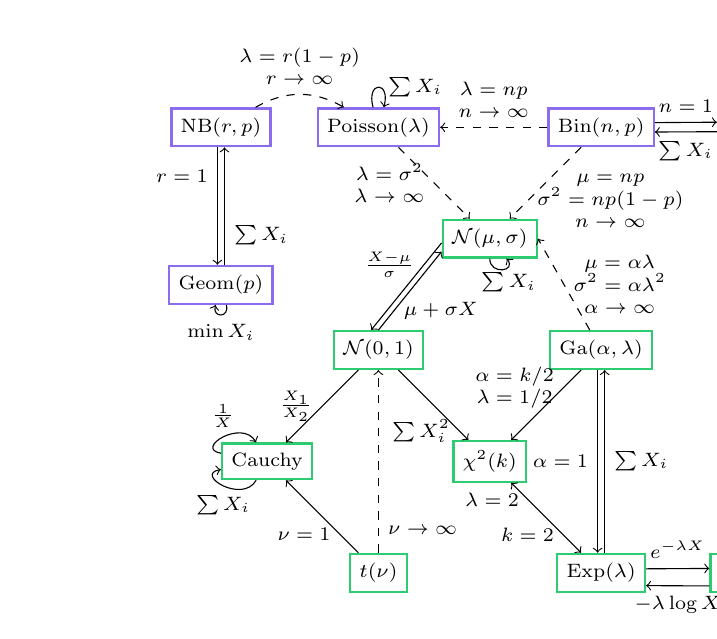
\begin{tikzpicture}[
	node distance = 2cm,
	dvertex/.style = {draw, rectangle, align=center, draw=discrete_highlight, thick},
  cvertex/.style = {draw, rectangle, align=center, draw=cont_highlight, thick},
]
\tikzstyle{every node}=[font=\scriptsize]

% Define vertices
\node[cvertex] (Normal) {\(\Normal(\mu, \sigma\))};
\node[dvertex, above left of=Normal] (Poisson) {\(\Poisson(\lambda)\)};
\node[dvertex, above right of=Normal] (Binomial) {\(\Bin(n, p)\)};
\node[dvertex, left of=Poisson] (NegBinomial) {\(\NB(r, p)\)};
\node[dvertex, below of=NegBinomial] (Geometric) {\(\Geom(p)\)};
\node[dvertex, right of=Binomial] (Bernoulli) {\(\Ber(p)\)};
\node[cvertex, below left of=Normal] (sNormal) {\(\Normal(0,1)\)};
\node[cvertex, below right of=Normal] (Gamma) {\(\Ga(\alpha, \lambda)\)};
\node[cvertex, below right of=sNormal] (ChiSquared) {\(\chi^2(k)\)};
\node[cvertex, below right of=ChiSquared] (Exponential) {\(\Exp(\lambda)\)};
\node[cvertex, below left of=ChiSquared] (StudentT) {\(t(\nu)\)};
\node[cvertex, below left of=sNormal] (Cauchy) {Cauchy};
\node[cvertex, right of=Exponential] (Uniform) {\(\Unif([a, b])\)};

% Draw edges with labels
\path[->] (NegBinomial.-100) edge node[left, align=center, near start]{\(r=1\)} (Geometric.100);
\path[->] (Geometric.80) edge node[right, align=center, near start]{\(\sum X_i\)} (NegBinomial.-80);
\path[->] (Geometric) edge[loop below, distance=5] node[below]{\(\min X_i\)} (Geometric);
\path[->, dashed] (NegBinomial) edge[bend left=30] node[above, align=center]{\(\lambda = r(1 - p)\) \\ \(r \to \infty\)} (Poisson);
\path[->] (Poisson) edge[loop above, distance=10] node[right]{\(\sum X_i\)} (Poisson);
\path[->, dashed] (Poisson) edge node[left, align=center]{\(\lambda = \sigma^2\) \\ \(\lambda \to \infty\)} (Normal);
\path[->] (Binomial.5) edge node[above]{\(n = 1\)} (Bernoulli.173);
\path[->] (Bernoulli.-174) edge node[below]{\(\sum X_i\)} (Binomial.-5);
\path[->, dashed] (Binomial) edge node[right, align=center, near end]{\(\mu = np\) \\ \(\sigma^2 = np(1 - p)\) \\ \(n \to \infty\)} (Normal);
\path[->, dashed] (Binomial) edge node[above, align=center]{\(\lambda = np\) \\ \(n \to \infty\)} (Poisson);
\path[->] (Normal.-175) edge node[left, near start]{\(\frac{X - \mu}{\sigma}\)} (sNormal.110);
\path[->] (sNormal.90) edge node[right, near start]{\(\mu + \sigma X\)} (Normal.-165);
\path[->] (Normal) edge[loop, in=-50, out=-90, looseness=5, distance=6] node[below, very near end]{\(\sum X_i\)} (Normal);
\path[->, dashed] (Gamma) edge node[right, align=center]{\(\mu = \alpha \lambda\) \\ \(\sigma^2 = \alpha \lambda^2\) \\ \(\alpha \to \infty\)} (Normal.0);
\path[->] (sNormal) edge node[left, very near end]{\(\sum X_i^2\)} (ChiSquared);
\path[->] (Gamma) edge[] node[left, align=center, near start]{\(\alpha = k/2\) \\ \(\lambda = 1/2\)} (ChiSquared);
\path[->] (Gamma.-100) edge node[left]{\(\alpha = 1\)} (Exponential.100);
\path[->] (Exponential.80) edge node[right]{\(\sum X_i\)} (Gamma.-80);
\path[<->] (ChiSquared) edge node[left, near start]{\(\lambda = 2\)} node[left, near end]{\(k = 2\)} (Exponential);
\path[->] (Exponential.5) edge node[above]{\(e^{-\lambda X}\)} (Uniform.175);
\path[->] (Uniform.-165) edge node[below]{\(-\lambda \log X\)} (Exponential.-16.5);
\path[->] (sNormal) edge node[left]{\(\frac{X_1}{X_2}\)} (Cauchy);
\path[->] (StudentT) edge node[left, near start]{\(\nu = 1\)} (Cauchy);
\path[->, dashed] (StudentT) edge node[right, very near start]{\(\nu \to \infty\)} (sNormal);
\path[->] (Cauchy) edge[loop, in=-170, out=-120, distance=10] node[below]{\(\sum X_i\)} (Cauchy);
\path[->] (Cauchy) edge[loop, in=120, out=170, distance=10] node[above]{\(\frac{1}{X}\)} (Cauchy);
\end{tikzpicture}
\end{center}

\begin{theorem*}[Distribution statements (\(X_1, \ldots, X_n\) iid. \(\sim \Normal(\mu, \sigma^2)\))]
  \begin{itemize}
    \item \(\bar{X_n} \sim \Normal(\mu, \frac{1}{n}\sigma^2)\) and thus \(\frac{\bar{X_n} - \mu}{\sigma / \sqrt{n}} \sim \Normal(0, 1)\).
    \item \(\frac{n-1}{\sigma^2}S^2 = \frac{1}{\sigma^2}\sum_{i=1}^n(X_i - \bar{X_n})^2 \sim \chi^2(n-1)\).
    \item \(\bar{X_n}\) and \(S^2\) are independent.
    \item \(\frac{\bar{X_n} - \mu}{S / \sqrt{n}} = \frac{\frac{\bar{X_n} - \mu}{\sigma / \sqrt{n}}}{\sqrt{\frac{1}{n-1} \frac{n-1}{\sigma^2}S^2}} \sim t_{n-1}\)
  \end{itemize}
\end{theorem*}

\begin{definition*}[Gamma Function] \vspace{-5pt}
  \[\Gamma(\alpha) := \int_0^\infty u^{\alpha-1}e^{-u} \, du \quad (\alpha > 0)\]
\end{definition*}

\begin{definition*}[Memorylessness]
  \(X\) memoryless \(\stackrel{\text{def}}{\iff} \P(X \geq s + t \mid X \geq s) = \P(X \geq t)\)
\end{definition*}

\section{Analysis Stuff}
\begin{definition*}[Derivative and integration rules]
  Linearity: \((\alpha \cdot f(x) + g(x))' = \alpha \cdot f'(x) + g'(x)\) \\
  Product rule: \((f \cdot g)'(x) = f'(x)\cdot g(x) + f(x)\cdot g'(x)\) \\
  Quotient rule: \(\left(\frac{f}{g}\right)'(x) = \frac{f'(x)\cdot g(x) - f(x)\cdot g'(x)}{g(x)^2}\) \\
  Chain rule: \((f \circ g)'(x) = f'(g(x))\cdot g'(x)\) \\
  Inverse: \((f^{-1})'(y_0) = \frac{1}{f'(x_0)} = \frac{1}{f'(f^{-1}(y_0))}, \ y_0 = f(x_0)\) \\
  Part. Int.: \(\int f(x) g'(x) \,dx = f(x)g(x) - \int f'(x) g(x) \, dx\)
\end{definition*}

\begin{itemize}
    \item Choose $g'$: exp $\rightarrow$ trig $\rightarrow$ poly $\rightarrow$ inverse trig. $\rightarrow$ logs
    \item Choose $f$: logs $\rightarrow$ inverse trig. $\rightarrow$ poly $\rightarrow$ trig $\rightarrow$ exp
    \item Sometimes it is necessary to multiply by $1$. \\ E.g.: $\int \ln x \ \,dx = \int \ln x \cdot 1 \ \,dx \Rightarrow f(x) = \ln x, \ g'(x) = 1$.
\end{itemize}

\begin{definition*}[Substitution] \vspace{-7pt}
    \[\int_{\phi(a)}^{\phi(b)} f(x) \,dx = \int_a^b f(\phi(t)) \phi'(t) dt = (F \circ \phi)(b) - (F \circ \phi)(a)\]
    since $F'=f$ then $f(\phi(t))\phi'(t) = (F \circ \phi)'(t)$.
\end{definition*}

\subsection{Series}
\begin{itemize}
  \item Geometric: $\sum_{n = 0}^\infty q^n = \frac{1}{1 - q}$ if $|q| < 1$
  \item Harmonic: $\sum_{n = 1}^\infty \frac{1}{n}$ diverges
  \item Telescope: $\sum_{n = 0}^\infty \frac{1}{n(n + 1)} = 1$
  \item $\exp(z) := \sum_{n = 0}^\infty \frac{z^n}{n!} = \lim_{n\to\infty}(1 + \frac{z}{n})^n = e^z$
  \item $\zeta(s) = \sum_{n=1}^\infty \frac{1}{n^s}$ converges $s > 1 \ (\frac{1}{1 - \frac{1}{2^{s-1}}})$
  \item $\text{p}(z) = \sum_{k = 0}^\infty c_kz^k$ conv. abs. $|z| < \rho = \frac{1}{\limsup |c_k|^{1/k}}$
\end{itemize}
\begin{tabularx}{\linewidth}{XX}
  \toprule
  $\sum\limits_{i=1}^n i = \frac{n(n+1)}{2}$ & $\sum\limits_{i=1}^n i^2 = \frac{n(n+1)(2n + 1)}{6}$ \\
  $\sum\limits_{i=1}^n i^3 = \frac{n^2(n+1)^2}{4}$ & $\sum\limits_{i=1}^\infty \frac{1}{n^2} = \frac{\pi^2}{6}$ \\
  \bottomrule
\end{tabularx}

\subsection{Logarithm Rules}
\renewcommand{\arraystretch}{1}
\begin{tabularx}{\linewidth}{XX}
  $\ln(1) = 0$ & $\ln(e) = 1$ \\
  $\ln(xy) = \ln(x) + \ln(y)$ & $\ln(x/y) = \ln(x) - \ln(y)$ \\
  $\ln(x^y) = y \cdot \ln(x)$ & $x^\alpha \cdot x^\beta = x^{\alpha + \beta}$ \\
  $(x^\alpha)^\beta = x^{\alpha \cdot \beta}$ & $\frac{x - 1}{x} \leq \ln(x) \leq x - 1$ \\
  $\ln(1 + x^\alpha) \leq \alpha x$ & $\log_\alpha(x) = \frac{\ln(x)}{\ln(\alpha)}$
\end{tabularx}

\subsection{Integral and Derivative Listing}
\begin{tabular}{c|c}
  $\mathbf{F(x)}$ & $\mathbf{f(x)}$ \\
  \midrule
  $c$ & $0$ \\
  $x^a$ & $a \cdot x^{a - 1}$ \\
  $\frac{1}{a+1} x^{a + 1}$ & $x^a$ \\
  $\frac{1}{a \cdot (n + 1)} (ax + b)^{n + 1}$ & $(ax + b)^n$ \\
  $\frac{x^{a + 1}}{a + 1}$ & $x^a, \ a \neq -1$ \\
  $\frac{1}{x}$ & $-\frac{1}{x^2}$ \\
  $\sqrt{x}$ & $\frac{1}{2\sqrt{x}}$ \\
  $\sqrt[n]{x}$ & $\frac{1}{n}x^{\frac{1}{n} - 1}$ \\
  $\frac{2}{3}x^{\frac{3}{2}}$ & $\sqrt{x}$ \\
  $\frac{n}{n+1} x^{\frac{1}{n} + 1}$ & $\sqrt[n]{x}$ \\
  $e^x$ & $e^x$ \\
  $\ln(|x|)$ & $\frac{1}{x}$ \\
  $\log_a(|x|)$ & $\frac{1}{x \ln(a)} = \log_a(e^\frac{1}{x})$ \\
  $\sin(x)$ & $\cos(x)$ \\
  $\frac{1}{2} (x + \sin(x) \cos(x))$ & $\cos^2(x)$ \\
  $\frac{1}{4}(\frac{1}{3}\sin(3x) + 3\sin(x))$ & $\cos^3(x)$ \\
  $-\cos(x)$ & $\sin(x)$ \\
  $\frac{1}{2} (x - \sin(x) \cos(x))$ & $\sin^2(x)$ \\
  $\frac{1}{4}(\frac{1}{3}\cos(3x) - 3\cos(x))$ & $\sin^3(x)$ \\
  $\ln\left(\left|\tan\left(\frac{x}{2}\right)\right|\right)$ & $\frac{1}{\sin(x)}$ \\
  $\ln\left(\left|\tan(\frac{x}{2} + \frac{\pi}{4})\right|\right)$ & $\frac{1}{\cos(x)}$ \\
  $\tan(x) = \frac{\sin(x)}{\cos(x)}$ & $\frac{1}{\cos^2(x)} = 1 + \tan^2(x)$ \\
  $\cot(x) = \frac{\cos(x)}{\sin(x)}$ & $\frac{1}{-\sin^2(x)}$ \\
  $a^{cx}$ & $a^{cx} \cdot c \ln(a)$ \\
  $\frac{ax}{c} - \frac{ad-bc}{c^2} \ln |cx +d|$ & $\frac{ax+b}{cx+d}$ \\
  $- x \cos (x) + \sin(x)$ & $x \sin (x)$ \\
  $x \sin(x) + \cos (x)$ & $x \cos (x)$ \\
  $-\frac{1}{a} \cos(ax + b)$ & $\sin(ax + b)$ \\
  $\frac{1}{a} \sin(ax + b)$ & $\cos(ax + b)$ \\
  $\sin(ax + b)$ & $a\cos(ax + b)$ \\
  $x^x$ & $x^x \cdot (1 + \ln(x)), \ x > 0$ \\
  $(x^x)^x$ & $(x^x)^x (x + 2x \ln(x)), \ x > 0$ \\
  $x^{x^x}$ & $x^{x^x} (x^{x - 1} + \ln(x) \cdot x^x (1 + \ln(x)))$ \\
  $\sqrt{\pi}$ & $\int_{-\infty}^\infty e^{-x^2} \,dx$ \\
  $\frac{1}{f(x)}$ & $\frac{-f'(x)}{(f(x))^2}$ \\
  $\ln(| f(x) |)$ & $\frac{f'(x)}{f(x)}$ \\
  $\frac{1}{2}(f(x))^2$ & $f'(x) f(x)$ \\
\end{tabular}

\subsection{Important Functions}
\begin{center}
  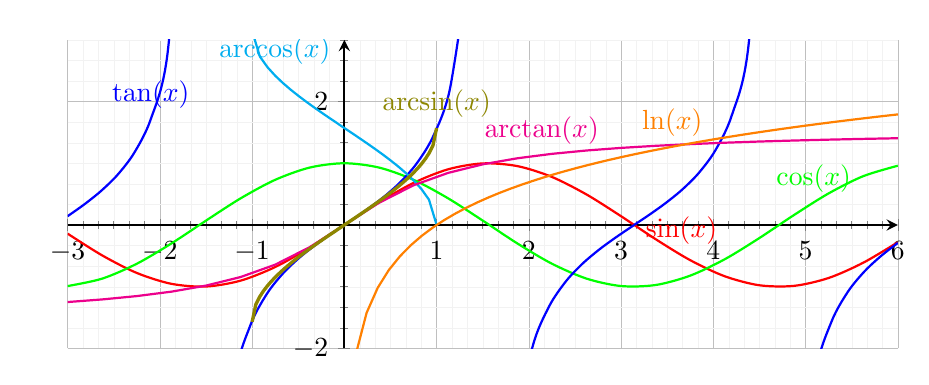
\begin{tikzpicture}
      \begin{axis}[
          axis lines = middle,
          domain = -3:6,
          ymin = -2,
          ymax = 3,
          width = \linewidth,
          height = 5.5cm,
          style = thick,
          grid = both,
          grid style = {line width=.1pt, draw=gray!10},
          major grid style = {line width=.2pt,draw=gray!50},
          minor tick num = 5,
          restrict y to domain=-10:10,
      ]
      
      \addplot[red, smooth]{sin(deg(x))} node[pos=0.75] (endofplotsquare1) {};
      \node [above,color=red] at (endofplotsquare1) {$\sin(x)$};

      \addplot[green, smooth]{cos(deg(x))} node[pos=0.9] (endofplotsquare2) {};
      \node [above,color=green] at (endofplotsquare2) {$\cos(x)$};

      \addplot[blue, smooth, samples=51]{tan(deg(x))} node[pos=0.05] (endofplotsquare3) {};
      \node [above,color=blue] at (endofplotsquare3) {$\tan(x)$};
      
      \addplot[cyan, domain=-1:1]{acos(x)/180*pi} node[pos=0.2] (endofplotsquare4) {};
      \node [above,color=cyan] at (endofplotsquare4) {$\arccos(x)$};

      \addplot[magenta] {atan(x)/180*pi} node[pos=0.6] (endofplotsquare5) {};
      \node [above,color=magenta] at (endofplotsquare5) {$\arctan(x)$};

      \addplot[olive, domain=-1:1, samples=51, style=very thick]{asin(x)/180*pi} node[pos=1] (endofplotsquare6) {};
      \node [above,color=olive] at (endofplotsquare6) {$\arcsin(x)$};

      \addplot[orange, domain=0.001:6, samples=51]{ln(x)} node[pos=0.8] (endofplotsquare7) {};
      \node [above,color=orange] at (endofplotsquare7) {$\ln(x)$};

      \end{axis}
  \end{tikzpicture}
\end{center}

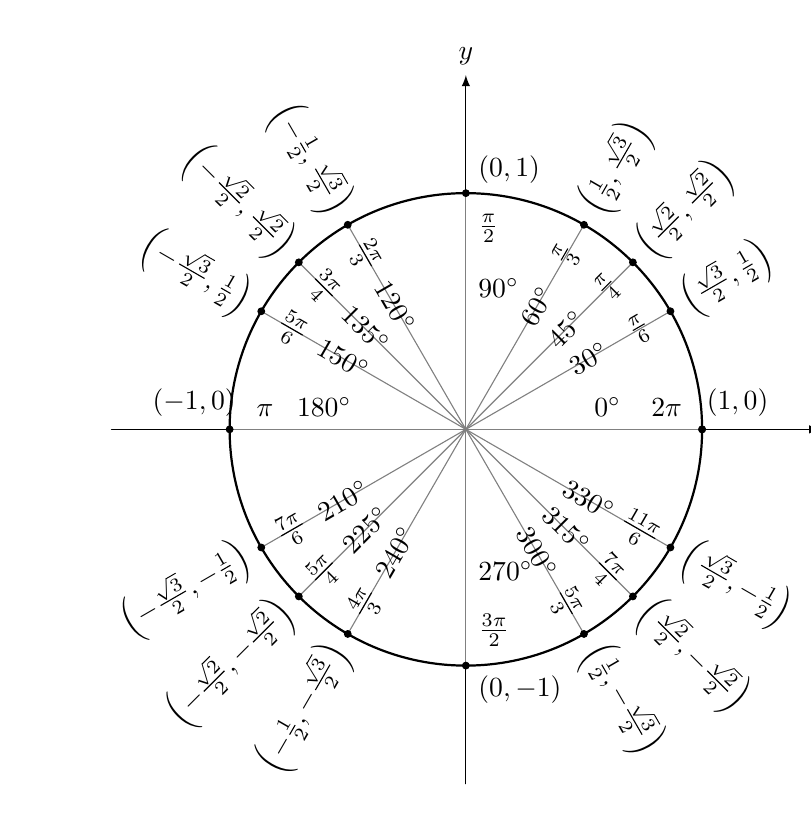
\begin{tikzpicture}[scale=3,cap=round,>=latex]
  \draw[->] (-1.5cm,0cm) -- (1.5cm,0cm) node[right,fill=white] {$x$}; % x axis
  \draw[->] (0cm,-1.5cm) -- (0cm,1.5cm) node[above,fill=white] {$y$}; % y axis
  
  % draw the unit circle
  \draw[thick] (0cm,0cm) circle(1cm);
  
  \foreach \x in {45,135, 225,315,0,30,...,360} { % <-- bissectrices added
    \draw[gray] (0cm,0cm) -- (\x:1cm); % lines from center to point
    \filldraw[black] (\x:1cm) circle(0.4pt); % dots at each point
  }
  
  % for the first and fourth quadrants
  \foreach \adeg/\radtext/\xc/\yc in {
    30/\frac{\pi}{6}/\frac{\sqrt{3}}{2}/\frac{1}{2},
    45/\frac{\pi}{4}/\frac{\sqrt{2}}{2}/\frac{\sqrt{2}}{2},
    60/\frac{\pi}{3}/\frac{1}{2}/\frac{\sqrt{3}}{2},
    300/\frac{5\pi}{3}/\frac{1}{2}/-\frac{\sqrt{3}}{2},
    315/\frac{7\pi}{4}/\frac{\sqrt{2}}{2}/-\frac{\sqrt{2}}{2},
    330/\frac{11\pi}{6}/\frac{\sqrt{3}}{2}/-\frac{1}{2}
  }
  {
    \draw (\adeg:0.6cm) node[rotate around={\adeg:(0,0)}] {$\adeg^\circ$}; % <-- rotate around key used
    \draw (\adeg:0.85cm) node[rotate around={\adeg:(0,0)}] {$\radtext$}; % <-- rotate around key used
    \draw (\adeg:1.025cm) node[rotate around={\adeg:(0,0)}, anchor=west] {$\left(\xc,\yc\right)$}; % <-- rotate around key used, radius changed, anchor key used
  }

  % for the second and third quadrants
  \foreach \adeg/\radtext/\xc/\yc in {
    120 / \frac{2\pi}{3} / -\frac{1}{2} / \frac{\sqrt{3}}{2},
    135 / \frac{3\pi}{4} / -\frac{\sqrt{2}}{2} / \frac{\sqrt{2}}{2},
    150 / \frac{5\pi}{6} / -\frac{\sqrt{3}}{2} / \frac{1}{2},
    210 / \frac{7\pi}{6} / -\frac{\sqrt{3}}{2} / -\frac{1}{2},
    225 / \frac{5\pi}{4} / -\frac{\sqrt{2}}{2} / -\frac{\sqrt{2}}{2},
    240 / \frac{4\pi}{3} / -\frac{1}{2} / -\frac{\sqrt{3}}{2}
  }
  {
    \draw (\adeg:0.6cm) node[rotate around={\adeg+180:(0,0)}] {$\adeg^\circ$}; % <-- rotate around key used
    \draw (\adeg:0.85cm) node[rotate around={\adeg+180:(0,0)}] {$\radtext$}; % <-- rotate around key used
    \draw (\adeg:1.025cm) node[rotate around={\adeg+180:(0,0)}, anchor=east] {$\left(\xc,\yc\right)$}; % <-- rotate around key used, radius changed, anchor key used
  }
  
  \foreach \adeg/\radtext/\xc/\yc in {0 / 2\pi / 1 / 0, 180 / \pi / -1 / 0}
  {
    \draw (\adeg:0.6cm) node[above=1pt] {$\adeg^\circ$};
    \draw (\adeg:0.85cm) node[above=1pt] {$\radtext$};
    \draw (\adeg:1.15cm) node[above=1pt] {$\left(\xc,\yc\right)$}; % <-- radius changed
  }
  
  \foreach \adeg/\radtext/\xc/\yc in {90 / \frac{\pi}{2} / 0 / 1, 270 / \frac{3\pi}{2} / 0 / -1}
  {
    \draw (\adeg:0.6cm) node[right=1pt] {$\adeg^\circ$};
    \draw (\adeg:0.85cm) node[right=1pt] {$\radtext$};
    \draw (\adeg:1.1cm) node[right=1pt] {$\left(\xc,\yc\right)$}; % <-- radius changed
  }
\end{tikzpicture}

\begin{tabularx}{\linewidth}{XX}
  \(\binom{n}{k} = \frac{n!}{(n-k)!k!}\) & \((x + y)^n = \sum\limits_{k=0}^n \binom{n}{k}x^{n-k}y^k\) \\
  \(x = \frac{-b \pm \sqrt{b^2 - 4ac}}{2a}\)
\end{tabularx}



\end{document}
